% Specific PFNs (Section 6) --- deep-dive deck.
% Window smoother, classification trees, localized PFN + the bias/variance figure.
% Standalone mini-deck, same metropolis style as ../presentation.tex.
% Build with: make   (tectonic)
\documentclass[aspectratio=169,10pt]{beamer}

\usetheme{metropolis}
\metroset{progressbar=frametitle, numbering=fraction, block=fill}

\usepackage[T1]{fontenc}
\usepackage{booktabs}
\usepackage{amsmath,amssymb}
\usepackage{tikz}
\usetikzlibrary{positioning,arrows.meta,fit,backgrounds,calc,matrix,decorations.pathreplacing}
\usepackage{pgfplots}
\pgfplotsset{compat=1.18}
\usepackage{xcolor}

% --- palette (identical to the main deck) ----------------------------------
\definecolor{accent}{HTML}{C1121F}
\definecolor{ink}{HTML}{2B2D42}
\definecolor{muted}{HTML}{6C757D}
\definecolor{good}{HTML}{2A9D8F}
\definecolor{biasc}{HTML}{2A6F97}
\definecolor{localc}{HTML}{5BA3D0}   % light blue = "Localized TabPFN" in Fig. 1
\setbeamercolor{frametitle}{bg=ink}
\setbeamercolor{background canvas}{bg=white}
\setbeamercolor{normal text}{fg=ink, bg=white}
\setbeamercolor{progress bar}{fg=accent}
\setbeamercolor{alerted text}{fg=accent}

\newcommand{\hl}[1]{{\color{accent}\textbf{#1}}}
\newcommand{\gd}[1]{{\color{good}\textbf{#1}}}
\newcommand{\mut}[1]{{\color{muted}#1}}
\newcommand{\cit}[1]{{\scriptsize\color{muted}[#1]}}

\title{Insights on Specific PFNs}
\subtitle{Window smoother, classification trees \& the localized PFN \;\cit{Nagler '23, \S6}}
\author{\underline{Gurmeher} Singh Puri \;\&\; Salih \underline{Bora} Öztürk}
\institute{Group 4 \;\textperiodcentered\; FM4SD Seminar \;\textperiodcentered\; SS26}
\date{}

\begin{document}

\maketitle

% ===========================================================================
% 1. Why this section / roadmap
% ===========================================================================
\begin{frame}[t]{From mechanisms to concrete predictors}

  \onslide<1->{\centering
    \S5 gave the \emph{rules}: variance dies from \hl{diminishing sensitivity};
    bias dies only with \hl{locality}.\\
    \S6 checks them on \hl{three concrete PFNs} --- each with a different bias story.\par}
  \vspace{0.7em}

  \onslide<2->{\centering
  \renewcommand{\arraystretch}{1.25}
  \begin{tabular}{@{}lcc@{}}
    \toprule
    \textbf{Predictor} & \textbf{Variance} & \textbf{Bias as $n\!\uparrow$} \\
    \midrule
    Window smoother \mut{\footnotesize(fixed $\theta$)}      & $\to 0$ & \hl{constant} \\
    Window smoother \mut{\footnotesize(shrinking $a_n$)}     & $\to 0$ & \gd{$\to 0$} \\
    Single classification tree                              & $\to 0$ & \hl{stuck} \\
    Tree ensemble \mut{\footnotesize(model averaging)}      & $\to 0$ & \gd{decreases} \\
    Transformer \mut{\footnotesize(TabPFN)}                 & $\to 0$ & decreases, then \hl{plateaus} \\
    \gd{Localized} TabPFN                                   & $\to 0$ & \gd{keeps decreasing} \\
    \bottomrule
  \end{tabular}\par}
  \vspace{0.6em}

  \onslide<3->{\centering
    {\footnotesize\mut{Variance is free everywhere. The whole table is really a story about \hl{bias}.}}\par}
\end{frame}

% ===========================================================================
% 2. The shared engine: Lemma 6.1 (generic smoother)
% ===========================================================================
\begin{frame}[t]{One lemma powers the variance for all of them \cit{Lem.\ 6.1}}

  \onslide<1->{\centering
    Both simple models are \hl{local averages} --- count labels inside a region $A_n(x)$ around $x$:
    \[
      q_{\theta}(y\mid x,\mathcal D_n)=
      \frac{\sum_{i=1}^n g(y,x,Y_i,X_i)}{\sum_{i=1}^n \mathbf 1\{X_i\in A_n(x)\}}.
    \]\par}
  \vspace{0.3em}

  \onslide<2->{\centering
    If the region holds a $n^{-\eta}$ share of the mass --- $n^{\eta}\Pr\{X_i\in A_n(x)\}\to c$ ---
    with $\eta\in(0,\tfrac12)$,\\[2pt]
    then the one-sample sensitivity bound \cit{Thm 5.2} holds with
    \;\hl{$\alpha=1-\eta$}\; and \;$L=4K/c$.\par}
  \vspace{0.6em}

  \onslide<3->{\centering
    {\gd{Consequence:}} any such local-average PFN has \hl{vanishing variance}
    \mut{(here $\alpha>\tfrac12$, so $n^{1/2-\alpha}\to0$).}\\[2pt]
    {\footnotesize\mut{Window smoother and trees both hit $\alpha=1$. So for both, only \emph{bias} is in question.}}\par}
\end{frame}

% ===========================================================================
% 3a. Window smoother --- the formula
% ===========================================================================
\begin{frame}[t]{1. Window smoother --- the formula}

  \onslide<1->{\centering
  \[
    q_\theta(y\mid x,\mathcal D_n)\;=\;
    \frac{\sum_{i}\, \alt<3->{\textcolor{accent}{\mathbf{1}(Y_i=y)}}{\textcolor{black!30}{\mathbf{1}(Y_i=y)}}\;
                       \alt<2->{\textcolor{good!55!black}{\mathbf{1}(\|X_i-x\|<\theta)}}{\textcolor{black!30}{\mathbf{1}(\|X_i-x\|<\theta)}}}
         {\sum_{i}\, \alt<2->{\textcolor{good!55!black}{\mathbf{1}(\|X_i-x\|<\theta)}}{\textcolor{black!30}{\mathbf{1}(\|X_i-x\|<\theta)}}}
  \]\par}
  \vspace{0.3em}

  \begin{columns}[T]
    \column{0.44\textwidth}
      \onslide<1->{\centering
      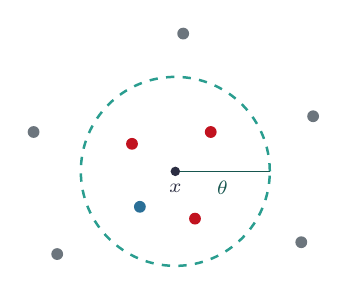
\begin{tikzpicture}[>=Latex]
        \draw[good, dashed, line width=0.9pt] (0,0) circle(1.2);
        \draw[good!55!black, line width=0.5pt] (0,0) -- (1.2,0) node[midway, below, font=\scriptsize]{$\theta$};
        \fill[ink] (0,0) circle(0.06);
        \node[ink, font=\scriptsize, below=0pt] at (0,-0.04){$x$};
        \fill[accent] (0.45,0.5) circle(0.075);
        \foreach \p in {(-0.55,0.35),(0.25,-0.6)} \fill[accent] \p circle(0.075);
        \fill[biasc] (-0.45,-0.45) circle(0.075);
        \foreach \p in {(1.75,0.7),(-1.8,0.5),(1.6,-0.9),(-1.5,-1.05),(0.1,1.75)} \fill[muted] \p circle(0.075);
      \end{tikzpicture}\\[4pt]
      {\scriptsize {\color{accent}$\bullet$}~label $y$\quad {\color{biasc}$\bullet$}~other\quad {\color{muted}$\bullet$}~outside}}
    \column{0.56\textwidth}
      {\footnotesize
      \onslide<1->{Average the labels of the points that land \textbf{inside a ball} of radius $\theta$ around $x$.\par}\medskip
      \onslide<2->{{\color{good!55!black}$\|X_i-x\|<\theta$}: inside the window (denominator counts them).\par}\medskip
      \onslide<3->{{\color{accent}$\mathbf{1}(Y_i=y)$}: of those, how many carry label $y$.\par}\medskip
      \onslide<4->{$q_\theta=\dfrac{\#\{\text{inside \& }y\}}{\#\{\text{inside}\}}=\dfrac{3}{4}$.\par}}
  \end{columns}
  \vspace{0.2em}
  \onslide<4->{\centering{\footnotesize\mut{$\theta^*$ is the KL-optimal bandwidth --- a hyperparameter \emph{tuned offline} on prior datasets.}}\par}
\end{frame}

% ===========================================================================
% 3b. Window smoother --- bias is constant
% ===========================================================================
\begin{frame}[t]{1. Window smoother --- a \emph{constant} bias}

  \onslide<1->{\centering
    With a \hl{fixed} bandwidth $\theta$, the bias does not depend on $n$:
    \[
      \mathbb E[q_\theta(y\mid x,\mathcal D_n)]-p_0(y\mid x)
      =\underbrace{\Pr_0(Y=y\mid \|X-x\|<\theta)}_{\text{average label in the window}}-\,p_0(y\mid x).
    \]\par}
  \vspace{0.4em}

  \onslide<2->{\centering
    The window has a \emph{fixed width}, so it always blurs the same neighbourhood
    $\Rightarrow$ \hl{bias is frozen}.\par}
  \vspace{0.3em}

  \onslide<3->{\centering
    {\gd{So this PFN learns from more data \emph{only} by shrinking variance}} ---
    bias stays put.\\[2pt]
    {\footnotesize\mut{Exactly the behaviour we will see plain TabPFN echo in the figure.}}\par}
  \vspace{0.6em}

  \onslide<4->{\centering
    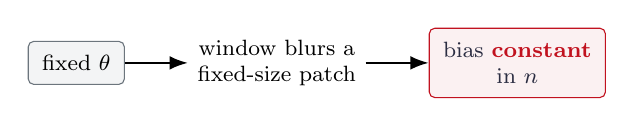
\begin{tikzpicture}[>=Latex, font=\footnotesize]
      \node[draw=muted, rounded corners=2pt, fill=muted!8, inner sep=5pt, align=center] (a)
        {fixed $\theta$};
      \node[right=8mm of a, align=center] (b) {window blurs a\\ fixed-size patch};
      \node[draw=accent, rounded corners=2pt, fill=accent!6, inner sep=5pt, right=8mm of b, align=center, text=ink] (c)
        {bias \hl{constant}\\ in $n$};
      \draw[->, line width=0.8pt] (a)--(b);
      \draw[->, line width=0.8pt] (b)--(c);
    \end{tikzpicture}
  \par}
\end{frame}

% ===========================================================================
% 3c. Window smoother --- shrinking window kills bias
% ===========================================================================
\begin{frame}[t]{1. Window smoother --- shrink the window, kill the bias}

  \onslide<1->{\centering
    Now let the radius \emph{shrink with $n$}: replace $\theta$ by $a_n\theta$ with a sequence $a_n$.
    \[
      q_\theta(y\mid x,\mathcal D_n)=
      \frac{\sum_i \mathbf 1(Y_i=y)\,\mathbf 1(\|X_i-x\|<\hl{$a_n$}\theta)}
           {\sum_i \mathbf 1(\|X_i-x\|<\hl{$a_n$}\theta)}.
    \]\par}
  \vspace{0.3em}

  \begin{columns}[T]
    \column{0.5\textwidth}
      \onslide<2->{\begin{block}{$a_n\uparrow$ (wider)}
        \footnotesize window swallows more $\Rightarrow$ blurs harder $\Rightarrow$
        \hl{bias grows}. \mut{A bad idea.}
      \end{block}}
    \column{0.5\textwidth}
      \onslide<3->{\begin{block}{$a_n\to 0$ (narrower)}
        \footnotesize if $p_0$ is smooth, the patch flattens $\Rightarrow$
        \gd{bias vanishes}.
      \end{block}}
  \end{columns}
  \vspace{0.6em}

  \onslide<4->{\centering
    The classical optimum is \;\hl{$a_n=n^{-1/(4+d)}$}\; \cit{kernel smoothing}:
    squared bias and variance both fall at rate $n^{-4/(4+d)}$.\\[2pt]
    {\footnotesize\mut{Now $\theta^*$ is just a prefactor, tuned to be optimal for prior datasets of \emph{any} size.}}\par}
  \vspace{0.3em}
  \onslide<5->{\centering
    {\gd{Lesson:}} to make bias vanish you must \hl{adapt the model to $n$} --- at the cost of more sensitivity.\par}
\end{frame}

% ===========================================================================
% 4a. Classification trees --- single tree
% ===========================================================================
\begin{frame}[t]{2. Classification trees --- one tree, stuck bias}

  \begin{columns}[T]
    \column{0.52\textwidth}
      \onslide<1->{\centering
      \[
        q_\theta(y\mid x,\mathcal D_n)=
        \sum_{j}\mathbf 1_{(\theta_j,\theta_{j+1}]}(x)\,
        \frac{\#\{Y_i=y,\ X_i\in(\theta_j,\theta_{j+1}]\}}{\#\{X_i\in(\theta_j,\theta_{j+1}]\}}
      \]
      \par}
      \onslide<1->{\centering
      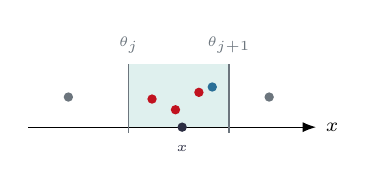
\begin{tikzpicture}[>=Latex, scale=0.85]
        \fill[good!15] (1.5,0) rectangle (3.0,0.95);
        \draw[->] (0,0) -- (4.3,0) node[right,font=\scriptsize]{$x$};
        \draw[muted, line width=0.5pt] (1.5,-0.08)--(1.5,0.95) node[above,font=\tiny,text=muted]{$\theta_j$};
        \draw[muted, line width=0.5pt] (3.0,-0.08)--(3.0,0.95) node[above,font=\tiny,text=muted]{$\theta_{j+1}$};
        \foreach \p in {(1.85,0.42),(2.55,0.52),(2.2,0.26)} \fill[accent] \p circle(0.07);
        \fill[biasc] (2.75,0.6) circle(0.07);
        \foreach \p in {(0.6,0.45),(3.6,0.45)} \fill[muted] \p circle(0.07);
        \fill[ink] (2.3,0) circle(0.07); \node[ink, font=\tiny] at (2.3,-0.32){$x$};
      \end{tikzpicture}}
    \column{0.48\textwidth}
      {\footnotesize
      \onslide<1->{Predict the \textbf{label-mix} of $x$'s bin --- the split points $\theta_j$ are the \hl{hyperparameters}, tuned offline.\par}\medskip
      \onslide<2->{Variance: \cit{Lem.\ 6.1} again gives $\alpha=1$ $\Rightarrow$ $\to 0$.\par}\medskip
      \onslide<3->{Bias $=\Pr_0(Y=y\mid X\in\text{bin})-p_0(y\mid x)$ --- \hl{independent of $n$}.\par}}
      \medskip
      \onslide<4->{{\footnotesize\hl{Why stuck?} To shrink bias you'd grow the number of splits $S$ with $n$ --- but the model is \emph{frozen} at inference. You cannot add parameters.}\par}
  \end{columns}
\end{frame}

% ===========================================================================
% 4b. Classification trees --- BMA ensemble
% ===========================================================================
\begin{frame}[t]{2. Classification trees --- an ensemble that \emph{does} learn}

  \onslide<1->{\centering
    Keep the trees frozen, but \hl{average many of them}, weighted by how well each fits:
    \[
      q_\theta=\sum_{k=1}^K q_{\theta_k}\,\underbrace{w(\mathcal D_n;\theta_k)}_{\propto\,\exp\{-\mathrm{BIC}_k\}},
      \qquad \mathrm{BIC}_k=-2\!\sum_i\log q_{\theta_k}(Y_i\mid X_i)+S\log n.
    \]\par}
  \vspace{0.3em}

  \begin{columns}[T]
    \column{0.46\textwidth}
      \onslide<2->{\centering
      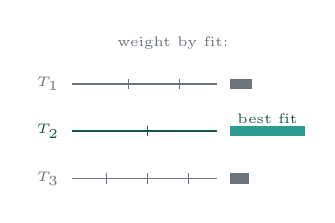
\begin{tikzpicture}[>=Latex, scale=0.8, font=\tiny]
        \node[muted] at (1.6,2.15){weight by fit:};
        \draw[muted] (0,1.5)--(2.3,1.5); \draw[muted](0.9,1.42)--(0.9,1.58);\draw[muted](1.7,1.42)--(1.7,1.58);
        \node[muted, left] at (-0.05,1.5){$T_1$};
        \fill[muted] (2.5,1.42) rectangle (2.85,1.58);
        \draw[good!55!black, line width=0.8pt] (0,0.75)--(2.3,0.75); \draw[good!55!black](1.2,0.67)--(1.2,0.83);
        \node[good!55!black, left] at (-0.05,0.75){$T_2$};
        \fill[good] (2.5,0.67) rectangle (3.7,0.83);
        \draw[muted] (0,0)--(2.3,0); \draw[muted](0.55,-0.08)--(0.55,0.08);\draw[muted](1.2,-0.08)--(1.2,0.08);\draw[muted](1.85,-0.08)--(1.85,0.08);
        \node[muted, left] at (-0.05,0){$T_3$};
        \fill[muted] (2.5,-0.08) rectangle (2.8,0.08);
        \node[good!55!black, font=\tiny] at (3.1,0.95){best fit};
      \end{tikzpicture}}
    \column{0.54\textwidth}
      {\footnotesize
      \onslide<3->{As $n$ grows, the BIC weights \hl{concentrate on the best-fitting trees} ---
      the ensemble drifts toward its strongest members.\par}\medskip
      \onslide<4->{{\gd{So the bias \emph{decreases} with $n$}}, approaching the best member's bias --- \emph{without} changing any parameter.\par}}
  \end{columns}
  \vspace{0.4em}

  \onslide<5->{\centering
    {\footnotesize\mut{This is \hl{implicit model selection / averaging} --- the very same trick multi-head attention pulls off in a transformer.}}\par}
\end{frame}

% ===========================================================================
% 5a. Localized PFN --- the construction
% ===========================================================================
\begin{frame}[t]{3. Localized PFN --- bolt locality onto any frozen net}

  \onslide<1->{\centering
    Transformers aren't local \cit{Thm 6.3}, so their bias plateaus.
    The fix needs \hl{no retraining} --- only change \emph{what you feed in}.\par}
  \vspace{0.6em}

  \onslide<1->{\centering
  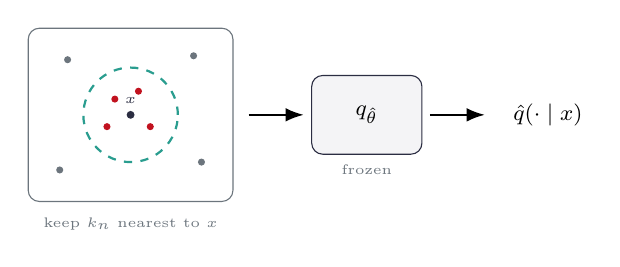
\begin{tikzpicture}[>=Latex, font=\footnotesize]
    \draw[muted, rounded corners] (0,0) rectangle (2.6,2.2);
    \draw[dashed, good, line width=0.8pt] (1.3,1.1) circle(0.6);
    \fill[ink] (1.3,1.1) circle(0.05); \node[ink,font=\tiny,above=-1pt] at (1.3,1.16){$x$};
    \foreach \p in {(1.1,1.3),(1.55,0.95),(1.4,1.4),(1.0,0.95)} \fill[accent] \p circle(0.045);
    \foreach \p in {(0.4,0.4),(2.2,0.5),(0.5,1.8),(2.1,1.85)} \fill[muted] \p circle(0.045);
    \node[muted, font=\tiny, anchor=north] at (1.3,-0.08){keep $k_n$ nearest to $x$};
    \draw[->,line width=0.8pt] (2.8,1.1)--(3.5,1.1);
    \node[draw=ink, fill=ink!5, rounded corners, minimum width=14mm, minimum height=10mm] (q) at (4.3,1.1) {$q_{\hat\theta}$};
    \node[muted,font=\tiny,below=0pt of q]{frozen};
    \draw[->,line width=0.8pt] (5.1,1.1)--(5.8,1.1);
    \node at (6.6,1.1) {$\hat q(\cdot\mid x)$};
  \end{tikzpicture}}
  \vspace{0.5em}

  \onslide<2->{\centering
    \textbf{1.} drop all but the $k_n$ nearest neighbours of $x$ $\to\mathcal D_n(x)$.\quad
    \textbf{2.} run the \emph{same} frozen $q_{\hat\theta}$ on $\mathcal D_n(x)$.\par}
  \vspace{0.3em}
  \onslide<3->{\centering
    {\gd{Why it works:}} zoom in near $x$ and the truth is $\approx$\hl{flat} $\Rightarrow$ easy to fit $\Rightarrow$ \gd{bias drops}.
    \mut{(It is a window smoother wrapped around the net.)}\par}
\end{frame}

% ===========================================================================
% 5b. Localized PFN --- the trade-off + schedule
% ===========================================================================
\begin{frame}[t]{3. Localized PFN --- the trade-off}

  \onslide<1->{\centering
    Nothing is free: fewer points $\Rightarrow$ a noisier average $\Rightarrow$ \hl{slightly more variance}.
    You hold the dial.\par}
  \vspace{0.7em}

  \onslide<1->{\centering
  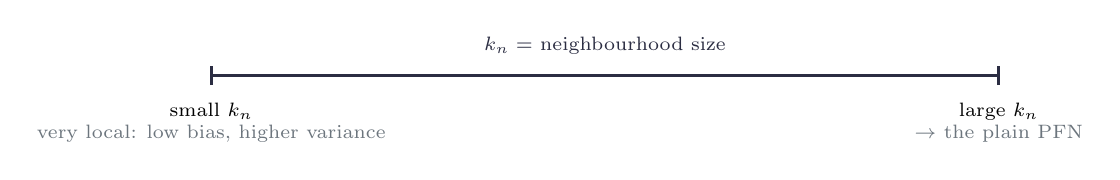
\begin{tikzpicture}[>=Latex, font=\footnotesize]
    \draw[line width=1.2pt, ink] (0,0) -- (10,0);
    \foreach \x in {0,10} \draw[ink, line width=1.2pt] (\x,-0.12)--(\x,0.12);
    \node[align=center, font=\scriptsize] at (0,-0.6) {small $k_n$\\ \mut{very local: low bias, higher variance}};
    \node[align=center, font=\scriptsize] at (10,-0.6) {large $k_n$\\ \mut{$\to$ the plain PFN}};
    \node[ink, font=\scriptsize, above] at (5,0.15){$k_n=$ neighbourhood size};
  \end{tikzpicture}}
  \vspace{0.9em}

  \onslide<2->{\centering
    The paper's schedule: \;\hl{$k_n=\min\{500,\ \lceil n^{4/(d+4)}\rceil\}$}\;
    \mut{($d=$ \#features)}.\par}
  \vspace{0.3em}
  \onslide<3->{\centering
    {\footnotesize The neighbourhood \emph{grows} with $n$ but \emph{shrinks relative} to the data ($k_n/n\to0$) ---
    so it stays local while still soaking up more points. \mut{(Same $n^{-1/(4+d)}$ optimal-smoothing rate as the window.)}}\par}
  \vspace{0.5em}
  \onslide<4->{\centering
    {\gd{Trade a little variance to break the bias floor}} --- and the figure shows exactly that.\par}
\end{frame}

% ===========================================================================
% 6. THE FIGURE --- Fig. 1, reproduced
% ===========================================================================
\begin{frame}[t]{The evidence: bias vs.\ variance, plain vs.\ localized \cit{Fig.\ 1}}

  \onslide<1->{\centering
    {\footnotesize 500 simulated sets, $p_0(1\mid X)=\tfrac12+\tfrac12\sin(\mathbf 1^\top X)$, $X\sim\mathcal N(\mathbf 0,I_5)$, pre-trained TabPFN.}\par}
  \vspace{0.2em}

  \begin{columns}[c]
    \column{0.5\textwidth}
      \centering
      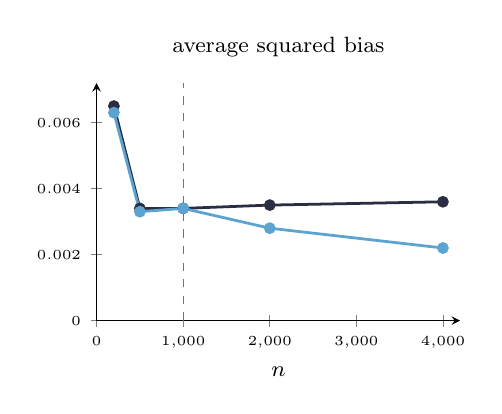
\begin{tikzpicture}
        \begin{axis}[
            width=6.2cm, height=4.6cm, title={\footnotesize average squared bias},
            xlabel={\footnotesize $n$}, xmin=0, xmax=4200, ymin=0, ymax=0.0072,
            scaled y ticks=false, ytick={0,0.002,0.004,0.006},
            yticklabel style={/pgf/number format/fixed, /pgf/number format/precision=3, font=\tiny},
            xtick={0,1000,2000,3000,4000}, xticklabel style={font=\tiny},
            tick align=outside, axis lines=left, every axis plot/.append style={line width=1pt, mark size=1.6pt}]
          \addplot[ink, mark=*] coordinates {(200,0.0065)(500,0.0034)(1000,0.0034)(2000,0.0035)(4000,0.0036)};
          \addplot[localc, mark=*] coordinates {(200,0.0063)(500,0.0033)(1000,0.0034)(2000,0.0028)(4000,0.0022)};
          \draw[dashed, muted] (axis cs:1000,0) -- (axis cs:1000,0.0072);
        \end{axis}
      \end{tikzpicture}
    \column{0.5\textwidth}
      \centering
      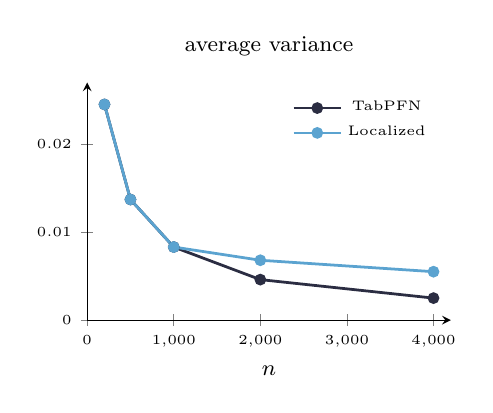
\begin{tikzpicture}
        \begin{axis}[
            width=6.2cm, height=4.6cm, title={\footnotesize average variance},
            xlabel={\footnotesize $n$}, xmin=0, xmax=4200, ymin=0, ymax=0.027,
            scaled y ticks=false, ytick={0,0.01,0.02},
            yticklabel style={/pgf/number format/fixed, /pgf/number format/precision=2, font=\tiny},
            xtick={0,1000,2000,3000,4000}, xticklabel style={font=\tiny},
            tick align=outside, axis lines=left, every axis plot/.append style={line width=1pt, mark size=1.6pt},
            legend style={font=\tiny, at={(0.97,0.97)}, anchor=north east, draw=none, fill=none}]
          \addplot[ink, mark=*] coordinates {(200,0.0245)(500,0.0137)(1000,0.0083)(2000,0.0046)(4000,0.0025)};
          \addlegendentry{TabPFN}
          \addplot[localc, mark=*] coordinates {(200,0.0245)(500,0.0137)(1000,0.0083)(2000,0.0068)(4000,0.0055)};
          \addlegendentry{Localized}
        \end{axis}
      \end{tikzpicture}
  \end{columns}
  \vspace{0.2em}

  \onslide<2->{\centering
    {\footnotesize
    \textbf{Bias (left):} {\color{ink}TabPFN} flattens after $n\!\approx\!1000$; {\color{localc}\textbf{localized}} \gd{keeps dropping}.\quad
    \textbf{Variance (right):} {\color{ink}TabPFN} falls $\sim\!1/n$; {\color{localc}\textbf{localized}} a touch \hl{higher} --- the cost.}\par}
\end{frame}

% ===========================================================================
% 7. Takeaways
% ===========================================================================
\begin{frame}[t]{What the three examples teach}

  \onslide<1->{\begin{itemize}\setlength\itemsep{0.7em}
    \item[\textcolor{accent}{1.}] \textbf{Window smoother} --- bias is whatever the \emph{fixed} window allows; constant in $n$
      unless you \hl{shrink the window with $n$}. Variance free.
    \item[\textcolor{accent}{2.}] \textbf{Classification trees} --- a single frozen tree has \hl{stuck} bias; an
      \gd{ensemble with model averaging} lets bias fall by \emph{selecting its best sub-models}.
    \item[\textcolor{accent}{3.}] \textbf{Localized PFN} --- a post-hoc \hl{$k_n$-nearest-neighbour wrapper} manufactures the
      locality the transformer lacks; \gd{bias keeps falling past 1000}, paying a little variance.
  \end{itemize}}
  \vspace{0.5em}

  \onslide<2->{\centering
    {\gd{The throughline:}} variance dies on its own; \hl{bias only falls if the model adapts to $n$} ---
    by shrinking a window, selecting sub-models, or localizing.\par}
\end{frame}

% ===========================================================================
\begin{frame}[standout]
  Variance is free.\\[6pt]
  Bias falls only when the predictor \emph{localizes} or \emph{selects} ---\\
  and we can bolt that on after training.
\end{frame}

\end{document}
